\documentclass[11pt,compress,t,notes=noshow, aspectratio=169, xcolor=table]{beamer}

\usepackage{../../style/lmu-lecture}
% Defines macros and environments
\usepackage[]{graphicx}
\usepackage[]{color}
% maxwidth is the original width if it is less than linewidth
% otherwise use linewidth (to make sure the graphics do not exceed the margin)
\makeatletter
\def\maxwidth{ %
\ifdim\Gin@nat@width>\linewidth
\linewidth
\else
\Gin@nat@width
\fi
}
\makeatother
%\usepackage[fontsize=10.5pt]{scrextend}
\definecolor{ggred}{rgb}{0.973, 0.463, 0.427}
\definecolor{ggblue}{rgb}{0, 0.749, 0.769}
\definecolor{fgcolor}{rgb}{0.345, 0.345, 0.345}
\newcommand{\hlnum}[1]{\textcolor[rgb]{0.686,0.059,0.569}{#1}}%
\newcommand{\hlstr}[1]{\textcolor[rgb]{0.192,0.494,0.8}{#1}}%
\newcommand{\hlcom}[1]{\textcolor[rgb]{0.678,0.584,0.686}{\textit{#1}}}%
\newcommand{\hlopt}[1]{\textcolor[rgb]{0,0,0}{#1}}%
\newcommand{\hlstd}[1]{\textcolor[rgb]{0.345,0.345,0.345}{#1}}%
\newcommand{\hlkwa}[1]{\textcolor[rgb]{0.161,0.373,0.58}{\textbf{#1}}}%
\newcommand{\hlkwb}[1]{\textcolor[rgb]{0.69,0.353,0.396}{#1}}%
\newcommand{\hlkwc}[1]{\textcolor[rgb]{0.333,0.667,0.333}{#1}}%
\newcommand{\hlkwd}[1]{\textcolor[rgb]{0.737,0.353,0.396}{\textbf{#1}}}%
\newcommand{\predvar}{Var\left[\hat{f}(\xv)\right]}
\let\hlipl\hlkwb

\usepackage{pdfpages}
\usepackage{framed}
\makeatletter
\newenvironment{kframe}{%
\def\at@end@of@kframe{}%
\ifinner\ifhmode%
\def\at@end@of@kframe{\end{minipage}}%
\begin{minipage}{\columnwidth}%
\fi\fi%
\def\FrameCommand##1{\hskip\@totalleftmargin \hskip-\fboxsep
\colorbox{shadecolor}{##1}\hskip-\fboxsep
% There is no \\@totalrightmargin, so:
\hskip-\linewidth \hskip-\@totalleftmargin \hskip\columnwidth}%
\MakeFramed {\advance\hsize-\width
\@totalleftmargin\z@ \linewidth\hsize
\@setminipage}}%
{\par\unskip\endMakeFramed%
\at@end@of@kframe}
\makeatother

\definecolor{shadecolor}{rgb}{.97, .97, .97}
\definecolor{messagecolor}{rgb}{0, 0, 0}
\definecolor{warningcolor}{rgb}{1, 0, 1}
\definecolor{errorcolor}{rgb}{1, 0, 0}
\newenvironment{knitrout}{}{} % an empty environment to be redefined in TeX

\usepackage{alltt}
\newcommand{\SweaveOpts}[1]{}  % do not interfere with LaTeX
\newcommand{\SweaveInput}[1]{} % because they are not real TeX commands
\newcommand{\Sexpr}[1]{}       % will only be parsed by R

\usepackage[english]{babel}
\usepackage[utf8]{inputenc}

\usepackage[export]{adjustbox}
\usepackage{dsfont}
\usepackage{verbatim}
\usepackage{amsmath}
\usepackage{amsfonts}
\usepackage{bm}
\usepackage{csquotes}
\usepackage{multirow}
\usepackage{longtable}
\usepackage{booktabs}
\usepackage{enumerate}
\usepackage[absolute,overlay]{textpos}
\usepackage{psfrag}
\usepackage{algorithm}
\usepackage{algpseudocode}
\usepackage{eqnarray}
\usepackage{arydshln}
\usepackage{tabularx}
\usepackage{placeins}
\usepackage{tikz}
\usepackage{setspace}
\usepackage{colortbl}
\usepackage{mathtools}
\usepackage{wrapfig}
\usepackage{bm}
\usepackage[backend=biber]{biblatex}

\usetikzlibrary{tikzmark, shapes,arrows,automata,positioning,calc,chains,trees,  shadows, decorations.pathreplacing}
\tikzset{
%Define standard arrow tip
>=stealth',
%Define style for boxes
punkt/.style={
rectangle,
rounded corners,
draw=black, very thick,
text width=6.5em,
minimum height=2em,
text centered},
% Define arrow style
pil/.style={
->,
thick,
shorten <=2pt,
shorten >=2pt,}
}

\usepackage{subfig}

\usepackage{bbm}
%\newcommand\hmmax{0}
%\newcommand\bmmax{0}
% basic latex stuff
\newcommand{\pkg}[1]{{\fontseries{b}\selectfont #1}} %fontstyle for R packages
\newcommand{\lz}{\vspace{0.5cm}} %vertical space
\newcommand{\dlz}{\vspace{1cm}} %double vertical space
\newcommand{\oneliner}[1] % Oneliner for important statements
{\begin{block}{}\begin{center}\begin{Large}#1\end{Large}\end{center}\end{block}}

% Latexmath Notation
% math spaces
\ifdefined\N                                                                
\renewcommand{\N}{\mathds{N}} % N, naturals
\else \newcommand{\N}{\mathds{N}} \fi 
\newcommand{\Z}{\mathds{Z}} % Z, integers
\newcommand{\Q}{\mathds{Q}} % Q, rationals
\newcommand{\R}{\mathds{R}} % R, reals
\ifdefined\C 
  \renewcommand{\C}{\mathds{C}} % C, complex
\else \newcommand{\C}{\mathds{C}} \fi
\newcommand{\continuous}{\mathcal{C}} % C, space of continuous functions
\newcommand{\M}{\mathcal{M}} % machine numbers
\newcommand{\epsm}{\epsilon_m} % maximum error

% counting / finite sets
\newcommand{\setzo}{\{0, 1\}} % set 0, 1
\newcommand{\setmp}{\{-1, +1\}} % set -1, 1
\newcommand{\unitint}{[0, 1]} % unit interval

% basic math stuff
\newcommand{\xt}{\tilde x} % x tilde
\newcommand{\argmax}{\operatorname{arg\,max}} % argmax
\newcommand{\argmin}{\operatorname{arg\,min}} % argmin
\newcommand{\argminlim}{\mathop{\mathrm{arg\,min}}\limits} % argmax with limits
\newcommand{\argmaxlim}{\mathop{\mathrm{arg\,max}}\limits} % argmin with limits  
\newcommand{\sign}{\operatorname{sign}} % sign, signum
\newcommand{\I}{\mathbb{I}} % I, indicator
\newcommand{\order}{\mathcal{O}} % O, order
\newcommand{\pd}[2]{\frac{\partial{#1}}{\partial #2}} % partial derivative
\newcommand{\floorlr}[1]{\left\lfloor #1 \right\rfloor} % floor
\newcommand{\ceillr}[1]{\left\lceil #1 \right\rceil} % ceiling

% sums and products
\newcommand{\sumin}{\sum\limits_{i=1}^n} % summation from i=1 to n
\newcommand{\sumim}{\sum\limits_{i=1}^m} % summation from i=1 to m
\newcommand{\sumjn}{\sum\limits_{j=1}^n} % summation from j=1 to p
\newcommand{\sumjp}{\sum\limits_{j=1}^p} % summation from j=1 to p
\newcommand{\sumik}{\sum\limits_{i=1}^k} % summation from i=1 to k
\newcommand{\sumkg}{\sum\limits_{k=1}^g} % summation from k=1 to g
\newcommand{\sumjg}{\sum\limits_{j=1}^g} % summation from j=1 to g
\newcommand{\meanin}{\frac{1}{n} \sum\limits_{i=1}^n} % mean from i=1 to n
\newcommand{\meanim}{\frac{1}{m} \sum\limits_{i=1}^m} % mean from i=1 to n
\newcommand{\meankg}{\frac{1}{g} \sum\limits_{k=1}^g} % mean from k=1 to g
\newcommand{\prodin}{\prod\limits_{i=1}^n} % product from i=1 to n
\newcommand{\prodkg}{\prod\limits_{k=1}^g} % product from k=1 to g
\newcommand{\prodjp}{\prod\limits_{j=1}^p} % product from j=1 to p

% linear algebra
\newcommand{\one}{\boldsymbol{1}} % 1, unitvector
\newcommand{\zero}{\mathbf{0}} % 0-vector
\newcommand{\id}{\boldsymbol{I}} % I, identity
\newcommand{\diag}{\operatorname{diag}} % diag, diagonal
\newcommand{\trace}{\operatorname{tr}} % tr, trace
\newcommand{\spn}{\operatorname{span}} % span
\newcommand{\scp}[2]{\left\langle #1, #2 \right\rangle} % <.,.>, scalarproduct
\newcommand{\mat}[1]{\begin{pmatrix} #1 \end{pmatrix}} % short pmatrix command
\newcommand{\Amat}{\mathbf{A}} % matrix A
\newcommand{\Deltab}{\mathbf{\Delta}} % error term for vectors

% basic probability + stats
\renewcommand{\P}{\mathds{P}} % P, probability
\newcommand{\E}{\mathds{E}} % E, expectation
\newcommand{\var}{\mathsf{Var}} % Var, variance
\newcommand{\cov}{\mathsf{Cov}} % Cov, covariance
\newcommand{\corr}{\mathsf{Corr}} % Corr, correlation
\newcommand{\normal}{\mathcal{N}} % N of the normal distribution
\newcommand{\iid}{\overset{i.i.d}{\sim}} % dist with i.i.d superscript
\newcommand{\distas}[1]{\overset{#1}{\sim}} % ... is distributed as ...

% machine learning
\newcommand{\Xspace}{\mathcal{X}} % X, input space
\newcommand{\Yspace}{\mathcal{Y}} % Y, output space
\newcommand{\nset}{\{1, \ldots, n\}} % set from 1 to n
\newcommand{\pset}{\{1, \ldots, p\}} % set from 1 to p
\newcommand{\gset}{\{1, \ldots, g\}} % set from 1 to g
\newcommand{\Pxy}{\mathbb{P}_{xy}} % P_xy
\newcommand{\Exy}{\mathbb{E}_{xy}} % E_xy: Expectation over random variables xy
\newcommand{\xv}{\mathbf{x}} % vector x (bold)
\newcommand{\xtil}{\tilde{\mathbf{x}}} % vector x-tilde (bold)
\newcommand{\yv}{\mathbf{y}} % vector y (bold)
\newcommand{\xy}{(\xv, y)} % observation (x, y)
\newcommand{\xvec}{\left(x_1, \ldots, x_p\right)^\top} % (x1, ..., xp) 
\newcommand{\Xmat}{\mathbf{X}} % Design matrix
\newcommand{\allDatasets}{\mathds{D}} % The set of all datasets
\newcommand{\allDatasetsn}{\mathds{D}_n}  % The set of all datasets of size n 
\newcommand{\D}{\mathcal{D}} % D, data
\newcommand{\Dn}{\D_n} % D_n, data of size n
\newcommand{\Dtrain}{\mathcal{D}_{\text{train}}} % D_train, training set
\newcommand{\Dtest}{\mathcal{D}_{\text{test}}} % D_test, test set
\newcommand{\xyi}[1][i]{\left(\xv^{(#1)}, y^{(#1)}\right)} % (x^i, y^i), i-th observation
\newcommand{\Dset}{\left( \xyi[1], \ldots, \xyi[n]\right)} % {(x1,y1)), ..., (xn,yn)}, data
\newcommand{\defAllDatasetsn}{(\Xspace \times \Yspace)^n} % Def. of the set of all datasets of size n 
\newcommand{\defAllDatasets}{\bigcup_{n \in \N}(\Xspace \times \Yspace)^n} % Def. of the set of all datasets 
\newcommand{\xdat}{\left\{ \xv^{(1)}, \ldots, \xv^{(n)}\right\}} % {x1, ..., xn}, input data
\newcommand{\ydat}{\left\{ \yv^{(1)}, \ldots, \yv^{(n)}\right\}} % {y1, ..., yn}, input data
\newcommand{\yvec}{\left(y^{(1)}, \hdots, y^{(n)}\right)^\top} % (y1, ..., yn), vector of outcomes
\renewcommand{\xi}[1][i]{\xv^{(#1)}} % x^i, i-th observed value of x
\newcommand{\yi}[1][i]{y^{(#1)}} % y^i, i-th observed value of y 
\newcommand{\xivec}{\left(x^{(i)}_1, \ldots, x^{(i)}_p\right)^\top} % (x1^i, ..., xp^i), i-th observation vector
\newcommand{\xj}{\xv_j} % x_j, j-th feature
\newcommand{\xjvec}{\left(x^{(1)}_j, \ldots, x^{(n)}_j\right)^\top} % (x^1_j, ..., x^n_j), j-th feature vector
\newcommand{\phiv}{\mathbf{\phi}} % Basis transformation function phi
\newcommand{\phixi}{\mathbf{\phi}^{(i)}} % Basis transformation of xi: phi^i := phi(xi)

%%%%%% ml - models general
\newcommand{\lamv}{\bm{\lambda}} % lambda vector, hyperconfiguration vector
\newcommand{\Lam}{\bm{\Lambda}}	 % Lambda, space of all hpos
% Inducer / Inducing algorithm
\newcommand{\preimageInducer}{\left(\defAllDatasets\right)\times\Lam} % Set of all datasets times the hyperparameter space
\newcommand{\preimageInducerShort}{\allDatasets\times\Lam} % Set of all datasets times the hyperparameter space
% Inducer / Inducing algorithm
\newcommand{\ind}{\mathcal{I}} % Inducer, inducing algorithm, learning algorithm 

% continuous prediction function f
\newcommand{\ftrue}{f_{\text{true}}}  % True underlying function (if a statistical model is assumed)
\newcommand{\ftruex}{\ftrue(\xv)} % True underlying function (if a statistical model is assumed)
\newcommand{\fx}{f(\xv)} % f(x), continuous prediction function
\newcommand{\fdomains}{f: \Xspace \rightarrow \R^g} % f with domain and co-domain
\newcommand{\Hspace}{\mathcal{H}} % hypothesis space where f is from
\newcommand{\fbayes}{f^{\ast}} % Bayes-optimal model
\newcommand{\fxbayes}{f^{\ast}(\xv)} % Bayes-optimal model
\newcommand{\fkx}[1][k]{f_{#1}(\xv)} % f_j(x), discriminant component function
\newcommand{\fh}{\hat{f}} % f hat, estimated prediction function
\newcommand{\fxh}{\fh(\xv)} % fhat(x)
\newcommand{\fxt}{f(\xv ~|~ \thetab)} % f(x | theta)
\newcommand{\fxi}{f\left(\xv^{(i)}\right)} % f(x^(i))
\newcommand{\fxih}{\hat{f}\left(\xv^{(i)}\right)} % f(x^(i))
\newcommand{\fxit}{f\left(\xv^{(i)} ~|~ \thetab\right)} % f(x^(i) | theta)
\newcommand{\fhD}{\fh_{\D}} % fhat_D, estimate of f based on D
\newcommand{\fhDtrain}{\fh_{\Dtrain}} % fhat_Dtrain, estimate of f based on D
\newcommand{\fhDnlam}{\fh_{\Dn, \lamv}} %model learned on Dn with hp lambda
\newcommand{\fhDlam}{\fh_{\D, \lamv}} %model learned on D with hp lambda
\newcommand{\fhDnlams}{\fh_{\Dn, \lamv^\ast}} %model learned on Dn with optimal hp lambda 
\newcommand{\fhDlams}{\fh_{\D, \lamv^\ast}} %model learned on D with optimal hp lambda 

% discrete prediction function h
\newcommand{\hx}{h(\xv)} % h(x), discrete prediction function
\newcommand{\hh}{\hat{h}} % h hat
\newcommand{\hxh}{\hat{h}(\xv)} % hhat(x)
\newcommand{\hxt}{h(\xv | \thetab)} % h(x | theta)
\newcommand{\hxi}{h\left(\xi\right)} % h(x^(i))
\newcommand{\hxit}{h\left(\xi ~|~ \thetab\right)} % h(x^(i) | theta)
\newcommand{\hbayes}{h^{\ast}} % Bayes-optimal classification model
\newcommand{\hxbayes}{h^{\ast}(\xv)} % Bayes-optimal classification model

% yhat
\newcommand{\yh}{\hat{y}} % yhat for prediction of target
\newcommand{\yih}{\hat{y}^{(i)}} % yhat^(i) for prediction of ith targiet
\newcommand{\resi}{\yi- \yih}

% theta
\newcommand{\thetah}{\hat{\theta}} % theta hat
\newcommand{\thetab}{\bm{\theta}} % theta vector
\newcommand{\thetabh}{\bm{\hat\theta}} % theta vector hat
\newcommand{\thetat}[1][t]{\thetab^{[#1]}} % theta^[t] in optimization
\newcommand{\thetatn}[1][t]{\thetab^{[#1 +1]}} % theta^[t+1] in optimization
\newcommand{\thetahDnlam}{\thetabh_{\Dn, \lamv}} %theta learned on Dn with hp lambda
\newcommand{\thetahDlam}{\thetabh_{\D, \lamv}} %theta learned on D with hp lambda
\newcommand{\mint}{\min_{\thetab \in \Theta}} % min problem theta
\newcommand{\argmint}{\argmin_{\thetab \in \Theta}} % argmin theta

% densities + probabilities
% pdf of x 
\newcommand{\pdf}{p} % p
\newcommand{\pdfx}{p(\xv)} % p(x)
\newcommand{\pixt}{\pi(\xv~|~ \thetab)} % pi(x|theta), pdf of x given theta
\newcommand{\pixit}[1][i]{\pi\left(\xi[#1] ~|~ \thetab\right)} % pi(x^i|theta), pdf of x given theta
\newcommand{\pixii}[1][i]{\pi\left(\xi[#1]\right)} % pi(x^i), pdf of i-th x 

% pdf of (x, y)
\newcommand{\pdfxy}{p(\xv,y)} % p(x, y)
\newcommand{\pdfxyt}{p(\xv, y ~|~ \thetab)} % p(x, y | theta)
\newcommand{\pdfxyit}{p\left(\xi, \yi ~|~ \thetab\right)} % p(x^(i), y^(i) | theta)

% pdf of x given y
\newcommand{\pdfxyk}[1][k]{p(\xv | y= #1)} % p(x | y = k)
\newcommand{\lpdfxyk}[1][k]{\log p(\xv | y= #1)} % log p(x | y = k)
\newcommand{\pdfxiyk}[1][k]{p\left(\xi | y= #1 \right)} % p(x^i | y = k)

% prior probabilities
\newcommand{\pik}[1][k]{\pi_{#1}} % pi_k, prior
\newcommand{\lpik}[1][k]{\log \pi_{#1}} % log pi_k, log of the prior
\newcommand{\pit}{\pi(\thetab)} % Prior probability of parameter theta

% posterior probabilities
\newcommand{\post}{\P(y = 1 ~|~ \xv)} % P(y = 1 | x), post. prob for y=1
\newcommand{\postk}[1][k]{\P(y = #1 ~|~ \xv)} % P(y = k | y), post. prob for y=k
\newcommand{\pidomains}{\pi: \Xspace \rightarrow \unitint} % pi with domain and co-domain
\newcommand{\pibayes}{\pi^{\ast}} % Bayes-optimal classification model
\newcommand{\pixbayes}{\pi^{\ast}(\xv)} % Bayes-optimal classification model
\newcommand{\pix}{\pi(\xv)} % pi(x), P(y = 1 | x)
\newcommand{\piv}{\bm{\pi}} % pi, bold, as vector
\newcommand{\pikx}[1][k]{\pi_{#1}(\xv)} % pi_k(x), P(y = k | x)
\newcommand{\pikxt}[1][k]{\pi_{#1}(\xv ~|~ \thetab)} % pi_k(x | theta), P(y = k | x, theta)
\newcommand{\pixh}{\hat \pi(\xv)} % pi(x) hat, P(y = 1 | x) hat
\newcommand{\pikxh}[1][k]{\hat \pi_{#1}(\xv)} % pi_k(x) hat, P(y = k | x) hat
\newcommand{\pixih}{\hat \pi(\xi)} % pi(x^(i)) with hat
\newcommand{\pikxih}[1][k]{\hat \pi_{#1}(\xi)} % pi_k(x^(i)) with hat
\newcommand{\pdfygxt}{p(y ~|~\xv, \thetab)} % p(y | x, theta)
\newcommand{\pdfyigxit}{p\left(\yi ~|~\xi, \thetab\right)} % p(y^i |x^i, theta)
\newcommand{\lpdfygxt}{\log \pdfygxt } % log p(y | x, theta)
\newcommand{\lpdfyigxit}{\log \pdfyigxit} % log p(y^i |x^i, theta)

% probababilistic
\newcommand{\bayesrulek}[1][k]{\frac{\P(\xv | y= #1) \P(y= #1)}{\P(\xv)}} % Bayes rule
\newcommand{\muk}{\bm{\mu_k}} % mean vector of class-k Gaussian (discr analysis) 

% residual and margin
\newcommand{\eps}{\epsilon} % residual, stochastic
\newcommand{\epsi}{\epsilon^{(i)}} % epsilon^i, residual, stochastic
\newcommand{\epsh}{\hat{\epsilon}} % residual, estimated
\newcommand{\yf}{y \fx} % y f(x), margin
\newcommand{\yfi}{\yi \fxi} % y^i f(x^i), margin
\newcommand{\Sigmah}{\hat \Sigma} % estimated covariance matrix
\newcommand{\Sigmahj}{\hat \Sigma_j} % estimated covariance matrix for the j-th class

% ml - loss, risk, likelihood
\newcommand{\Lyf}{L\left(y, f\right)} % L(y, f), loss function
\newcommand{\Lypi}{L\left(y, \pi\right)} % L(y, pi), loss function
\newcommand{\Lxy}{L\left(y, \fx\right)} % L(y, f(x)), loss function
\newcommand{\Lxyi}{L\left(\yi, \fxi\right)} % loss of observation
\newcommand{\Lxyt}{L\left(y, \fxt\right)} % loss with f parameterized
\newcommand{\Lxyit}{L\left(\yi, \fxit\right)} % loss of observation with f parameterized
\newcommand{\Lxym}{L\left(\yi, f\left(\bm{\tilde{x}}^{(i)} ~|~ \thetab\right)\right)} % loss of observation with f parameterized
\newcommand{\Lpixy}{L\left(y, \pix\right)} % loss in classification
\newcommand{\Lpiv}{L\left(y, \piv\right)} % loss in classification
\newcommand{\Lpixyi}{L\left(\yi, \pixii\right)} % loss of observation in classification
\newcommand{\Lpixyt}{L\left(y, \pixt\right)} % loss with pi parameterized
\newcommand{\Lpixyit}{L\left(\yi, \pixit\right)} % loss of observation with pi parameterized
\newcommand{\Lhxy}{L\left(y, \hx\right)} % L(y, h(x)), loss function on discrete classes
\newcommand{\Lr}{L\left(r\right)} % L(r), loss defined on residual (reg) / margin (classif)
\newcommand{\lone}{|y - \fx|} % L1 loss
\newcommand{\ltwo}{\left(y - \fx\right)^2} % L2 loss
\newcommand{\lbernoullimp}{\ln(1 + \exp(-y \cdot \fx))} % Bernoulli loss for -1, +1 encoding
\newcommand{\lbernoullizo}{- y \cdot \fx + \log(1 + \exp(\fx))} % Bernoulli loss for 0, 1 encoding
\newcommand{\lcrossent}{- y \log \left(\pix\right) - (1 - y) \log \left(1 - \pix\right)} % cross-entropy loss
\newcommand{\lbrier}{\left(\pix - y \right)^2} % Brier score
\newcommand{\risk}{\mathcal{R}} % R, risk
\newcommand{\riskbayes}{\mathcal{R}^\ast}
\newcommand{\riskf}{\risk(f)} % R(f), risk
\newcommand{\riskdef}{\E_{y|\xv}\left(\Lxy \right)} % risk def (expected loss)
\newcommand{\riskt}{\mathcal{R}(\thetab)} % R(theta), risk
\newcommand{\riske}{\mathcal{R}_{\text{emp}}} % R_emp, empirical risk w/o factor 1 / n
\newcommand{\riskeb}{\bar{\mathcal{R}}_{\text{emp}}} % R_emp, empirical risk w/ factor 1 / n
\newcommand{\riskef}{\riske(f)} % R_emp(f)
\newcommand{\risket}{\mathcal{R}_{\text{emp}}(\thetab)} % R_emp(theta)
\newcommand{\riskr}{\mathcal{R}_{\text{reg}}} % R_reg, regularized risk
\newcommand{\riskrt}{\mathcal{R}_{\text{reg}}(\thetab)} % R_reg(theta)
\newcommand{\riskrf}{\riskr(f)} % R_reg(f)
\newcommand{\riskrth}{\hat{\mathcal{R}}_{\text{reg}}(\thetab)} % hat R_reg(theta)
\newcommand{\risketh}{\hat{\mathcal{R}}_{\text{emp}}(\thetab)} % hat R_emp(theta)
\newcommand{\LL}{\mathcal{L}} % L, likelihood
\newcommand{\LLt}{\mathcal{L}(\thetab)} % L(theta), likelihood
\newcommand{\LLtx}{\mathcal{L}(\thetab | \xv)} % L(theta|x), likelihood
\newcommand{\logl}{\ell} % l, log-likelihood
\newcommand{\loglt}{\logl(\thetab)} % l(theta), log-likelihood
\newcommand{\logltx}{\logl(\thetab | \xv)} % l(theta|x), log-likelihood
\newcommand{\errtrain}{\text{err}_{\text{train}}} % training error
\newcommand{\errtest}{\text{err}_{\text{test}}} % test error
\newcommand{\errexp}{\overline{\text{err}_{\text{test}}}} % avg training error

% lm
\newcommand{\thx}{\thetab^\top \xv} % linear model
\newcommand{\olsest}{(\Xmat^\top \Xmat)^{-1} \Xmat^\top \yv} % OLS estimator in LM 

%%%%%% perturbed data
\usepackage{xifthen}
\newcommand{\pert}[3]{\ifthenelse{\equal{#2}{}}{\tilde{#1}}{\ifthenelse{\equal{#3}{}}{\tilde{#1}^{#2}}{\tilde{#1}^{#2|#3}}}}	% command to express that for #1 the subset #2 was perturbed given subset #3

%%%%%% marginalized functions
\newcommand{\fj}{f_j} % marginal function f_j, depending on feature j
\newcommand{\fnj}{f_{-j}} % marginal function f_{-j}, depending on all features but j
\newcommand{\fS}{f_S} % marginal function f_S depending on feature set S
\newcommand{\fnj}{f_{-S}} % marginal function f_{-S}, depending on all features but features in S
\newcommand{\fC}{f_C} % marginal function f_C depending on feature set C
\newcommand{\fhj}{\fh_j} % marginal function fh_j, depending on feature j
\newcommand{\fhnj}{\fh_{-j}} % marginal function fh_{-j}, depending on all features but j
\newcommand{\fhS}{\fh_S} % marginal function fh_S depending on feature set S
\newcommand{\fhnS}{\fh_{-S}} % marginal function fh_{-S}, depending on all features but features in S
\newcommand{\fhC}{\fh_C} % marginal function fh_C depending on feature set C
\newcommand{\XSmat}{\Xmat_S} % Design matrix subset
\newcommand{\XnSmat}{\Xmat__{-S}} % Design matrix subset without S
\newcommand{\XCmat}{\Xmat_C} % Design matrix subset
\newcommand{\Xnj}{\Xmat_{-j}} % Design matrix subset -j = {1, .., j-1, j+1, ..., p}

%%%%% Shapley values
\newcommand{\Scupj}{S \cup \{j\}} % coalition S but without player j
\newcommand{\Scupk}{S \cup \{k\}} % coalition S but without player k
\newcommand{\SsubP}{S \subseteq P} % coalition S subset of P
\newcommand{\SsubPnoj}{\SsubP \setminus \{j\}} % coalition S subset of P without player j
\newcommand{\SsubPnojk}{\SsubP \setminus \{j,k\}} % coalition S subset of P without player k
\newcommand{\phiij}{\hat{\phi}_j^{(i)}} % Shapley value for feature j and observation i

%%%%% LIME 
\newcommand{\Gspace}{\mathcal{G}} % Hypothesis space for surrogate model
\newcommand{\neigh}{\phi_{\xv}} % Proximity measure
\newcommand{\zv}{\mathbf{z}} % Sampled datapoints for surrogate
\newcommand{\Zspace}{\mathcal{Z}} % Space of sampled datapoints
\newcommand{\Gower}{d_G} % Gower distance


\newcommand{\indep}{\perp}
\newcommand{\Ind}{\mathcal{I}}

%new environments
\newenvironment{vbframe}  %frame with breaks and verbatim
{
\begin{frame}%[containsverbatim,allowframebreaks]
}
{
\end{frame}
}

% \newenvironment{vframe}  %frame with verbatim without breaks (to avoid numbering one slided frames)
% {
%  \begin{frame}[containsverbatim]
% }
% {
% \end{frame}
% }

\newenvironment{blocki}[1]   % itemize block
{
 \begin{block}{#1}\begin{itemize}
}
{
\end{itemize}\end{block}
}

\newenvironment{fragileframe}[2]{  %fragile frame with framebreaks
\begin{frame}[allowframebreaks, fragile, environment = fragileframe]
\frametitle{#1}
#2}
{\end{frame}}


\newcommand{\myframe}[2]{  %short for frame with framebreaks
\begin{frame}[allowframebreaks]
\frametitle{#1}
#2
\end{frame}}

\newcommand{\remark}[1]{
  \textbf{Remark:} #1
}


\newenvironment{deleteframe}
{
\begingroup
\usebackgroundtemplate{
\includegraphics[width=\paperwidth,height=\paperheight]{../style/color/red.png}}
 \begin{frame}
}
{
\end{frame}
\endgroup
}
\newenvironment{simplifyframe}
{
\begingroup
\usebackgroundtemplate{
\includegraphics[width=\paperwidth,height=\paperheight]{../style/color/yellow.png}}
 \begin{frame}
}
{
\end{frame}
\endgroup
}\newenvironment{draftframe}
{
\begingroup
\usebackgroundtemplate{
\includegraphics[width=\paperwidth,height=\paperheight]{../style/color/green.jpg}}
 \begin{frame}
}
{
\end{frame}
\endgroup
}
% https://tex.stackexchange.com/a/261480: textcolor that works in mathmode
\makeatletter
\renewcommand*{\@textcolor}[3]{%
  \protect\leavevmode
  \begingroup
    \color#1{#2}#3%
  \endgroup
}
\makeatother

% \makeatletter
% %\newcommand\notsotiny{\@setfontsize\notsotiny\@vipt\@viipt}
% \newcommand\notsotiny{\@setfontsize\notsotiny{6.31415}{7.1828}}
% \makeatother

\providecommand{\tightlist}{%
  \setlength{\itemsep}{0pt}\setlength{\parskip}{0pt}}

%\setbeamerfont{footnote}{size=\tiny}
\usepackage[hang,flushmargin]{footmisc}
\renewcommand*{\footnotelayout}{\tiny}
\renewcommand*{\thefootnote}{} %\fnsymbol{footnote}

% https://tex.stackexchange.com/questions/638616/beamer-frametitle-always-uppercase-for-text-but-not-for-href-or-url
\usepackage{textcase}

% https://stackoverflow.com/questions/377301/is-there-a-latex-command-to-make-text-all-lower-caps
%\usepackage[overload]{textcase}
%\setbeamertemplate{frametitle}{\MakeTextUppercase{\insertframetitle}}
%\setbeamertemplate{frametitle}{\expandafter\uppercase\expandafter\insertframetitle}

\setbeamertemplate{frametitle}{\MakeTextUppercase{\insertframetitle}}
\newcommand{\citebutton}[2]{%
\NoCaseChange{\resizebox{!}{9pt}{\protect\beamergotobutton{\href{#2}{#1}}}}%
}

%\setbeamertemplate{frametitle}{\expandafter\uppercase\expandafter\insertframetitle}
%\newcommand{\citebutton}[2]{%
%\href{#2}{\footnotesize\color{black!60}[#1]}
%\resizebox{!}{9pt}{\beamergotobutton{\lowercase{\href{#2}}{#1}}}% \MakeLowercase
%}
%\newcommand{\lit}[2]{\href{#2}{\footnotesize\color{black!60}[#1]}}

\newcommand{\lit}[2]{\href{#2}{\footnotesize\color{black!60}[#1]}}

\let\code=\texttt
\let\proglang=\textsf

\setkeys{Gin}{width=0.9\textwidth}

% https://tex.stackexchange.com/questions/30720/footnote-without-a-marker
% \makeatletter
% \def\blfootnote{\gdef\@thefnmark{}\@footnotetext}
% \makeatother

% https://tex.stackexchange.com/questions/357717/beamer-allowframebreaks-option-and-vertical-spacing-when-using-lists-itemize
% \setbeamertemplate{frametitle continuation}{%
%     (\insertcontinuationcount)%
%     \ifnum\insertcontinuationcount>1%
%     \vspace*{\topsep}%
%     \else%
%     %
%     \fi%
% }


\title{Interpretable Machine Learning}
% \author{LMU}
%\institute{\href{https://compstat-lmu.github.io/lecture_iml/}{compstat-lmu.github.io/lecture\_iml}}
\date{}

\bibliography{feature-importance}
%\usepackage{Sweave}
\begin{document}
	\newcommand{\titlefigure}{figure_man/feature-importance.png}
    \newcommand{\learninggoals}{
    	\item Underdstand how PFI is computed
    	\item Understanding strengths and weaknesses
    	\item Testing Importance}
	% Set style/preamble.Rnw as parent.
	
	% Load all R packages and set up knitr
	
	% This file loads R packages, configures knitr options and sets preamble.Rnw as 
	% parent file
	% IF YOU MODIFY THIS, PLZ ALSO MODIFY setup.Rmd ACCORDINGLY...
	
	% Defines macros and environments

	\lecturechapter{Permutation Feature Importance}
	\lecture{Interpretable Machine Learning}
	
	% ------------------------------------------------------------------------------

% \begin{frame}{Permutation Feature Importance Idea \citebutton{Breiman (2001)}{https://doi.org/10.1023/A:1010933404324}}

% In general, feature importance methods share two components
% \lz
% \begin{enumerate}
%   \item \textbf{Perturbation/Removal:} Generate predictions for which the feature of interest has been perturbed or removed.
%   \item \textbf{Performance Comparison:} Compare performance under perturbation/removal with the original model performance.
% \end{enumerate}
% \lz
% \textbf{Permutation Feature Importance Idea:} "Remove" the feature of interest $x_j$ by perturbing it such that it is uninformative. Therefore, resample the variable from its marginal distribution $\P(x_j)$, e.g. by randomly permuting observations in $x_j$.

% %\footnote[frame]{\fullcite{Breiman2001rf}}

% %\framebreak

% %\begin{figure}
% %  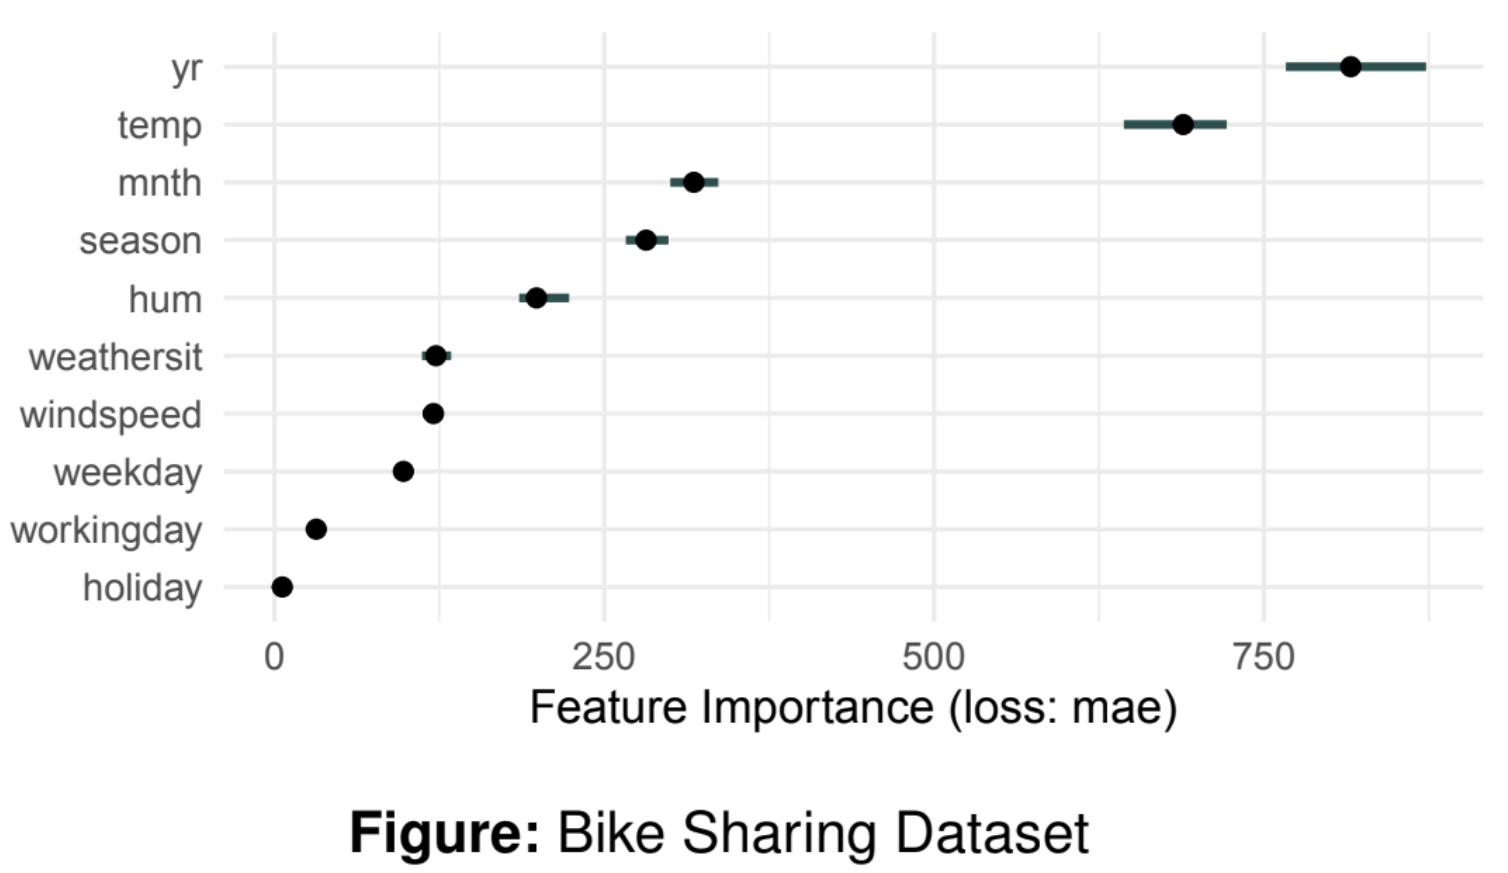
\includegraphics[width=0.75\textwidth]{figure_man/feature-importance.png}
% %\end{figure}

% %\vspace{-0.2cm}
% %\tiny{Fisher et al. (2018). All models are wrong but many are useful: Variable importance for black-box, proprietary, or misspecified prediction models, using model class reliance. arXiv preprint arXiv:1801.01489 (2018).}

% \end{frame}

\begin{frame}{Permutation Feature Importance (PFI) \citebutton{Breiman (2001)}{https://doi.org/10.1023/A:1010933404324}}

\textbf{Idea:} "Destroy" feature of interest $x_j$ by perturbing it such that it becomes uninformative, e.g., randomly permute observations in $x_j$ (marginal distribution $\P(x_j)$ stays the same).  %Therefore, resample the variable from its marginal distribution $\P(x_j)$, e.g. by randomly permuting observations in $x_j$.

PFI for features $x_S$ using test data $\D$:
\begin{itemize}
  \item Measure the error {\color{blue}\textbf{without permuting features}} and {\color{red}\textbf{with permuted feature values}} $\pert{x}{}{}_S$
  \item Repeat permuting the feature (e.g., $m$ times) and average the difference of both errors: 
$$\widehat{PFI}_S = \tfrac{1}{m} \textstyle\sum\nolimits_{k = 1}^{m} \riske (\fh, {\color{red}\pert{\D}{S}{}_{(k)}}) - \riske (\fh, {\color{blue}\D}), \text{ where }
\riske(\fh, \D) = \frac{1}{n} \sum\nolimits_{(x, y) \in \D}  L(\fh(x), y)$$
\end{itemize}
\pause
The data $\D$ where $x_S$ is replaced with $\pert{x}{S}{}$ is denoted as $\pert{\D}{S}{}$.\\
Example of permuting feature $x_S$ with $S = \{1\}$ and $m=6$:

% TODO: update to new notation
\begin{center}
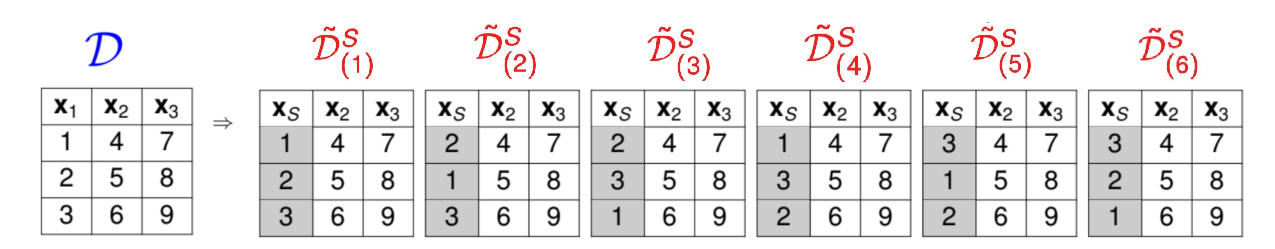
\includegraphics[width=0.75\textwidth]{figure_man/permuted-fv.pdf}
\end{center}

\vspace*{0.2cm}
{\scriptsize{Note: 
The $S$ in $x_S$ refers to a \textbf{S}ubset of features for which we are interested in their effect on the prediction.\\
Here: We calculate the feature importance for one feature at a time $|S| = 1$.}\par}

\end{frame}



% \begin{columns}
%   \begin{column}{0.5\textwidth}
%     \only<1-3,5-7>{$\hspace{36pt}{\color{white}\riske(\fh, {\color{red}\pert{\D}{S}{}_{(k)}}) - \riske(\fh, {\color{blue}\D})}$}
%   \only<4>{$\hspace{36pt}\riske(\fh, {\color{red}\pert{\D}{S}{}_{(k)}}) - \riske(\fh, {\color{blue}\D}),$ where 
% $\riske(\fh, \D) =$ \scalebox{0.7}{$\frac{1}{n} \sum\nolimits_{(x, y) \in \D}$} $\scriptstyle L(\fh(x), y)$}
% % $\scriptstyle\riske(\fh, \D) =$ \scalebox{0.7}{$\frac{1}{n} \sum\nolimits_{(x, y) \in \D}$} $\scriptstyle L(\fh(x), y)$}
% %   \only<5-6>{$\hspace{36pt}{\color{white}\riske(\fh, {\color{red}\pert{\D}{S}{}_{(k)}}) - \riske(\fh, {\color{blue}\D})}$}
  
%   \begin{center}
%   \only<1>{\includegraphics[page=2, trim=0pt 5pt 0 66pt, clip, width=\textwidth]{figure_man/pfi_demo2}}%
%   \only<2>{\includegraphics[page=3, trim=0pt 5pt 0 66pt, clip, width=\textwidth]{figure_man/pfi_demo2}}%
%   \only<3-4>{\includegraphics[page=4, trim=0pt 5pt 0 66pt, clip, width=\textwidth]{figure_man/pfi_demo2}}%
%   \only<5>{\includegraphics[page=5, trim=0pt 5pt 0 66pt, clip, width=\textwidth]{figure_man/pfi_demo2}}%
%   \only<6>{\includegraphics[page=6, trim=0pt 5pt 0 66pt, clip, width=\textwidth]{figure_man/pfi_demo2}}%
%   \only<7>{\includegraphics[page=7, trim=0pt 5pt 0 66pt, clip, width=\textwidth]{figure_man/pfi_demo2}}%
%   \end{center}
%   \end{column}
%   \begin{column}{0.5\textwidth}
  
%   \begin{itemize}
%     \only<1-2>{\item[1.]\textbf{Perturbation:} Sample feature values from the distribution of $x_S$ ($P(X_S)$). \newline $\Rightarrow$ Randomly permute feature $x_S$. Replace the original feature with the permuted feature $\pert{x}{}{}_S$ and create data with permuted feature   $\pert{\D}{S}{}$.}
%     \only<2>{\item[2.] \textbf{Prediction:} Make predictions for both data, i.e., $\D$ and $\pert{\D}{S}{}$.}
%     \only<3-4>{\item[3.] \textbf{Aggregation:}
%       \begin{itemize}
%         \item Compute the loss for each observation in both data sets.
%       \end{itemize}}
%     \only<5>{\item[3.] \textbf{Aggregation:}
%       \begin{itemize}
%         \item Compute the loss for each observation in both data sets.
%       \item Take the difference of both losses $\Delta L$ for each observation.
%       \end{itemize}}
%      \only<6>{\item[3.] \textbf{Aggregation:}
%       \begin{itemize}
%         \item Compute the loss for each observation in both data sets.
%         \item Take the difference of both losses $\Delta L$ for each observation.
%         \item Average this change in loss across all observations.
%       \end{itemize}}
%     \only<7>{\item[3.] \textbf{Aggregation:}
%       \begin{itemize}
%         \item Compute the loss for each observation in both data sets.
%         \item Take the difference of both losses $\Delta L$ for each observation.
%         \item Average this change in loss across all observations.
%         \item Also, average over multiple repetitions, if available.
%       \end{itemize}}
%   \end{itemize}
%   \end{column}
% \end{columns}



\begin{frame}{Permutation Feature Importance}

  \only<1-4>{$\hspace{80pt}{\color{white}\riske(\fh, {\color{red}\pert{\D}{S}{}_{(k)}}) - \riske(\fh, {\color{blue}\D})}$}
  \only<5-6>{$\hspace{80pt}\riske(\fh, {\color{red}\pert{\D}{S}{}_{(k)}}) - \riske(\fh, {\color{blue}\D})$}
% $\scriptstyle\riske(\fh, \D) =$ \scalebox{0.7}{$\frac{1}{n} \sum\nolimits_{(x, y) \in \D}$} $\scriptstyle L(\fh(x), y)$}
%   \only<5-6>{$\hspace{36pt}{\color{white}\riske(\fh, {\color{red}\pert{\D}{S}{}_{(k)}}) - \riske(\fh, {\color{blue}\D})}$}
  
  \begin{center}
  \only<1>{\includegraphics[page=2, trim=0pt 5pt 0 66pt, clip, width=0.7\textwidth]{figure_man/pfi_demo2}}%
  \only<2>{\includegraphics[page=3, trim=0pt 5pt 0 66pt, clip, width=0.7\textwidth]{figure_man/pfi_demo2}}%
  \only<3>{\includegraphics[page=4, trim=0pt 5pt 0 66pt, clip, width=0.7\textwidth]{figure_man/pfi_demo2}}%
  \only<4>{\includegraphics[page=5, trim=0pt 5pt 0 66pt, clip, width=0.7\textwidth]{figure_man/pfi_demo2}}%
  \only<5>{\includegraphics[page=6, trim=0pt 5pt 0 66pt, clip, width=0.7\textwidth]{figure_man/pfi_demo2}}%
  \only<6>{\includegraphics[page=7, trim=0pt 5pt 0 66pt, clip, width=0.7\textwidth]{figure_man/pfi_demo2}}%
  \end{center}
  
  \begin{itemize}
    \only<1-2>{\item[1.]\textbf{Perturbation:} Sample feature values from the distribution of $x_S$ ($P(X_S)$). \newline 
    $\Rightarrow$ Randomly permute feature $x_S$ \\
    $\Rightarrow$ Replace original feature with permuted feature $\pert{x}{}{}_S$ and create data $\pert{\D}{S}{}$ containing $\pert{x}{}{}_S$} 
    \only<2>{\item[2.] \textbf{Prediction:} Make predictions for both data, i.e., $\D$ and $\pert{\D}{S}{}$}
    \only<3->{\item[3.] \textbf{Aggregation:}}
      \begin{itemize}
        \item<3-> Compute the loss for each observation in both data sets
        \item<4-> Take the difference of both losses $\Delta L$ for each observation
        \item<5-> Average this change in loss across all observations
        \only<5>{\\ Note: This is equivalent to computing $\riske$ on both data sets and taking the difference}
        \item<6-> Repeat pertubation and average over multiple repetitions%, if available
      \end{itemize}
    % \only<3-4>{\item[3.] \textbf{Aggregation:}
    %   \begin{itemize}
    %     \item Compute the loss for each observation in both data sets.
    %   \end{itemize}}
    % \only<5>{\item[3.] \textbf{Aggregation:}
    %   \begin{itemize}
    %     \item Compute the loss for each observation in both data sets.
    %   \item Take the difference of both losses $\Delta L$ for each observation.
    %   \end{itemize}}
    %  \only<6>{\item[3.] \textbf{Aggregation:}
    %   \begin{itemize}
    %     \item Compute the loss for each observation in both data sets.
    %     \item Take the difference of both losses $\Delta L$ for each observation.
    %     \item Average this change in loss across all observations.
    %   \end{itemize}}
    % \only<7>{\item[3.] \textbf{Aggregation:}
    %   \begin{itemize}
    %     \item Compute the loss for each observation in both data sets.
    %     \item Take the difference of both losses $\Delta L$ for each observation.
    %     \item Average this change in loss across all observations.
    %     \item Also, average over multiple repetitions, if available.
    %   \end{itemize}}
  \end{itemize}
\end{frame}

\begin{frame}{Example: Bike Sharing Dataset}

\begin{center}
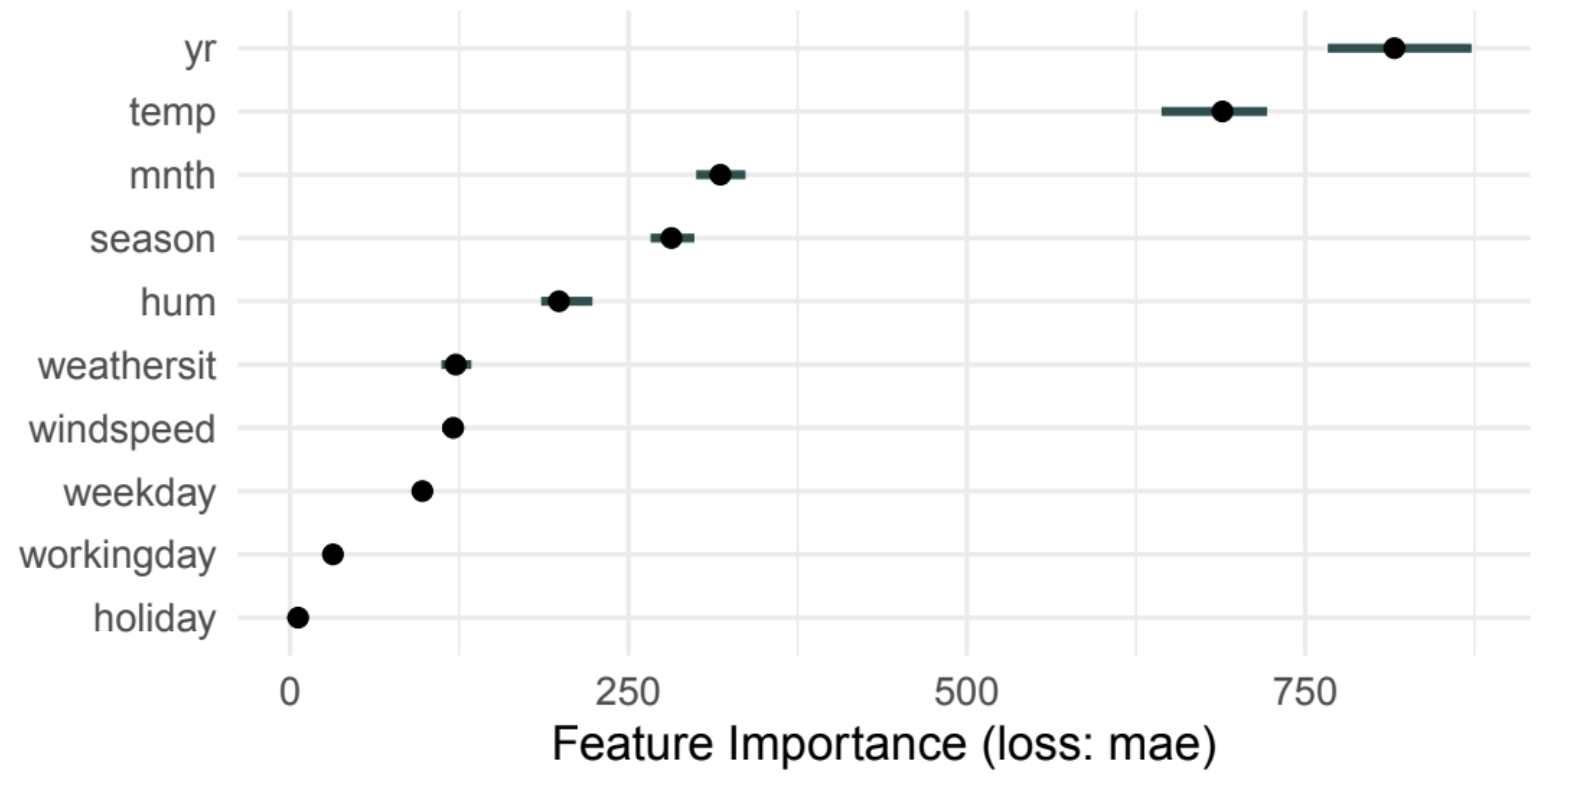
\includegraphics[width=0.6\textwidth]{figure_man/bike-sharing02.png}
\end{center}

\textbf{Interpretation:}

\begin{itemize}
 \item Year (\code{yr}) and Temperature (temp) are most important features
 %Features such as weekday also contribute to the performance.
 \item Destroying information about \code{yr} by permuting it increases mean absolute error of model by 816
 \item $5 \%$ and $95 \%$ quantile of repetitions due multiple permutations are shown as error bars
\end{itemize}
\end{frame}

\begin{frame}{Comments on PFI}
 \begin{itemize}[<+->]
 \itemsep1em
  \item Interpretation: PFI is the increase of model error when feature's information is destroyed
  \item Results can be unreliable due to random permutations \\
  $\Rightarrow$ Solution: Average results over multiple repetitions
  \item Permuting features despite correlation with other features can lead to unrealistic combinations of feature values (since under dependence $\P(x_j,x_{-j}) \neq \P(x_j) \P(x_{-j})$) $\leadsto$ Extrapolation issue
  \item PFI automatically includes importance of interaction effects with other features \\
  $\Rightarrow$ Permutation also destroys information of interactions where permuted feature is involved\\
  $\Rightarrow$ Importance of all interactions with the permuted feature are contained in PFI score %Not only importance of permuted feature is contained but also importance of all interactions with that feature
  \item Interpretation of PFI depends on whether training or test data is used
 \end{itemize}
\end{frame}

%TODO: Simplify example
\begin{frame}{Comments on PFI - Extrapolation}
 
%\textbf{Example:} Let $y = x_3 + \epsilon_y$ with $\epsilon_y \sim N(0, 0.1)$ where $x_1$, $x_2 := x_1 + \epsilon_1$ are highly correlated ($x_1 \sim N(0,1), \epsilon_1 \sim N(0, 0.01)$). Let $x_3, x_4 \sim N(0,1)$ be noisy features are independent.
 
 \textbf{Example:} Let $y = x_3 + \epsilon_y$ with $\epsilon_y \sim N(0, 0.1)$ where $x_1 :=  \epsilon_1$, $x_2 := x_1 + \epsilon_2$ are highly correlated ($\epsilon_1 \sim N(0,1), \epsilon_2 \sim N(0, 0.01)$) and $x_3 := \epsilon_3$, $x_4 := \epsilon_4$,  with $\epsilon_3, \epsilon_4 \sim N(0,1)$. All noise terms are independent.
 Fitting a LM yields $\fh(\xv) \approx 0.3 x_1 - 0.3 x_2 + x_3$.
\pause

%\begin{figure}
% \hfill
%   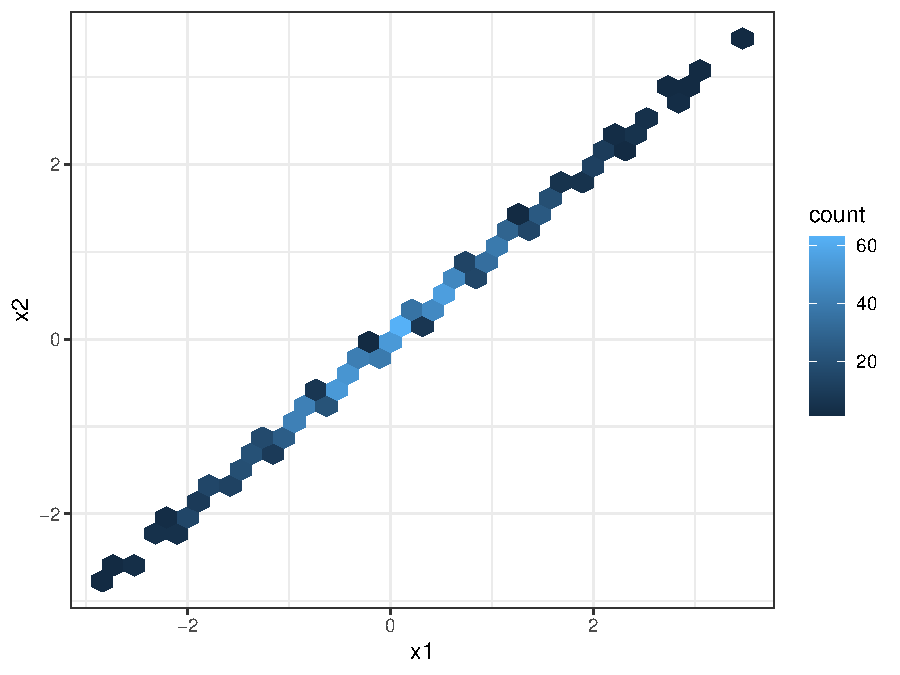
\includegraphics[width=0.3\linewidth]{figure_man/pfi_hexbin_pre.pdf}\hfill
%   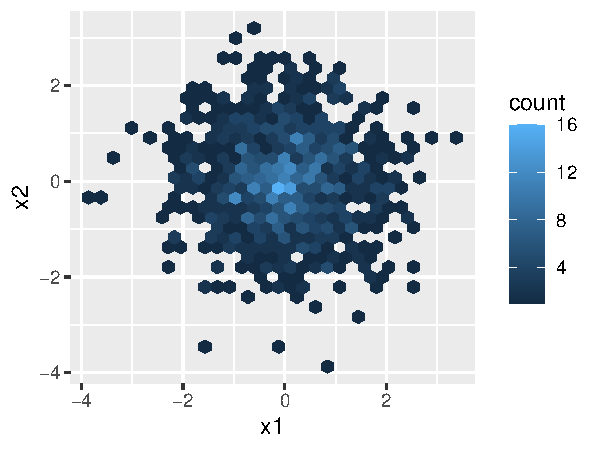
\includegraphics[width=0.3\linewidth]{figure_man/pfi_hexbin_post.pdf} \hfill
%   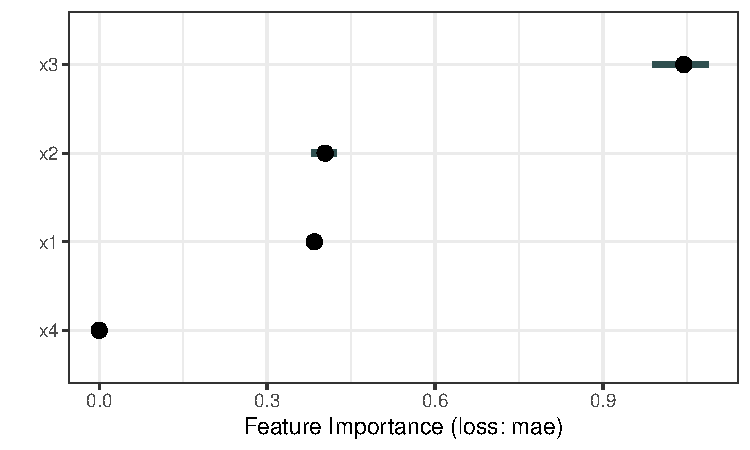
\includegraphics[width=0.39\linewidth]{figure_man/pfi_extrapolation.pdf} \hfill
\centerline{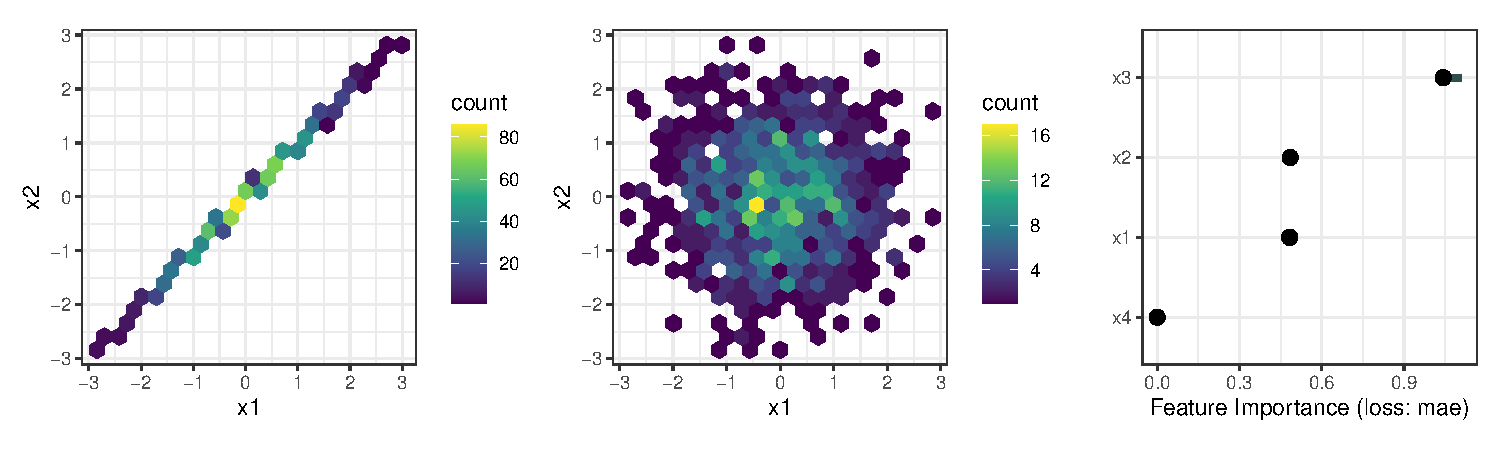
\includegraphics[width=0.9\linewidth]{figure_man/pfi_hexbin_extrapolation.pdf}}
\centerline{Hexbin plot of $x_1, x_2$ before permuting $x_1$ (left), after permuting $x_1$ (center), and PFI scores (right)}
\lz\pause
% \caption{Density plot for $x_1, x_2$ before permuting $x_1$ (left) and after permuting $x_1$ (center). Right: PFI including $.05$ to $.95$ quantiles.}
%\end{figure}
% 
$\Rightarrow$ $x_1$ and $x_2$ should be irrelevant for the prediction $\fh(\xv)$ for $\{\xv: \P(\xv) > 0\}$ as $0.3 x_1 - 0.3 x_2 \approx 0$ \\
$\Rightarrow$ PFI evaluates model on unrealistic obs. outside $\P(\xv)$ $\leadsto$ $x_1$, $x_2$ are considered relevant (PFI $> 0$)
%$\Rightarrow$ Since PFI evaluates the model on unrealistic observations, the features $x_1$ and $x_2$ are nevertheless considered relevant

 \end{frame}

\begin{frame}{Comments on PFI - Interactions}

\textbf{Example:} Let $x_1, \dots, x_4$ be independently and uniformly sampled from $\{-1, 1\}$ and 
$$y:= x_1 x_2 + x_3 + \epsilon_Y \text{ with } \epsilon_Y \sim N(0, 1)$$

\begin{columns}[T, totalwidth = \textwidth]
\begin{column}{0.5\textwidth}

Fitting a LM yields $\fh(x) \approx x_1 x_2 + x_3$.\\
\lz\pause
Although $x_3$ alone contributes as much to the performance as $x_1$ and $x_2$ jointly, all three are considered equally relevant.\\
\lz
$\Rightarrow$ PFI does not fairly attribute the performance to the individual features.

\end{column}
\begin{column}{0.5\textwidth}
\centering
  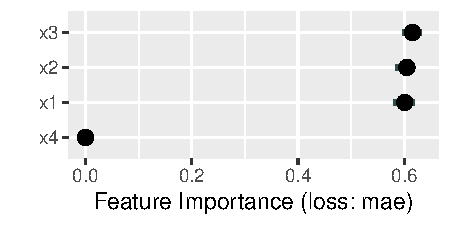
\includegraphics[width=\linewidth]{figure_man/pfi_interactions.pdf}
\end{column}
\end{columns}


\end{frame}

\begin{frame}{Comments on PFI - Test vs. Training data}

\textbf{Example:} $x_1, \dots, x_{20}, y$ are independently sampled from $\mathcal{U} (-10, 10)$. An \texttt{xgboost} model with default hyperparameters is fit on a small training set of $50$ observations. The model overfits heavily.\\

\begin{figure}
  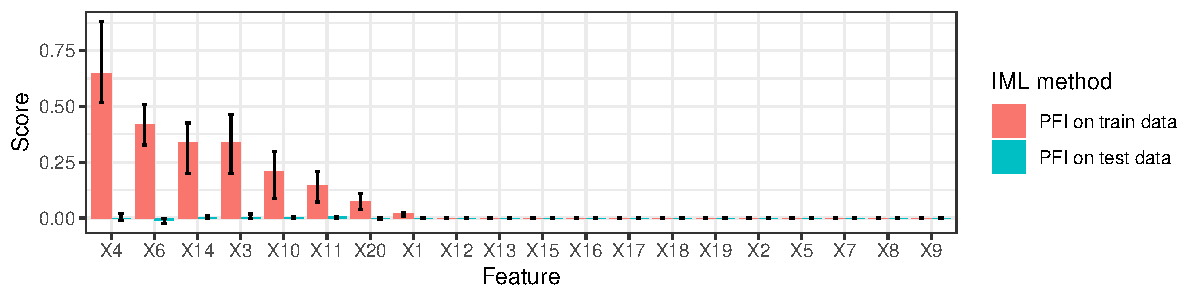
\includegraphics[width=0.9\linewidth]{figure_man/pfi_test_vs_train.pdf}
  \caption{While PFI on test data considers all features to be irrelevant, PFI on train data exposes the features on which the model overfitted.}
\end{figure}

\pause

Why? PFI can only be nonzero if the permutation breaks a dependence in the data. Spurious correlations help the model perform well on train data, but are not present in the test data.\\
$\Rightarrow$ If you are interested in which features help the model to generalize, apply PFI on test data.
  
\end{frame}

\begin{frame}{Implications of PFI}

Can we get insight into whether ...

\begin{enumerate}
    \item<1-> the feature $x_j$ is causal for the prediction?
    \begin{itemize}
      \item $PFI_j \neq 0$ $\Rightarrow$ model relies on $x_j$
      \item As the training vs test data example demonstrates, the contraposition does not hold
    \end{itemize}
    \item<2-> the variable $x_j$ contains prediction-relevant information?
    \begin{itemize}
      \item $x_{j}$ is dependent of $y$ or it's covariates $x_{-j}$ or both (due to extrapolation) $\Rightarrow$ $PFI_j > 0$ 
      \item $x_{j}$ is not exploited by model (regardless of whether it is useful for $y$ or not) $\Rightarrow$ $PFI_j = 0$  %irrespective of whether the feature is useful or not
    \end{itemize}
    \item<3-> the model requires access to $x_j$ to achieve it's prediction performance?    
    \begin{itemize}
      \item As the extrapolation example demonstrates, such insight is not possible
\end{itemize}
\end{enumerate}
\end{frame}


\begin{frame}{Testing Importance (PIMP) \citebutton{Altmann et al. (2010)}{https://doi.org/10.1093/bioinformatics/btq134}}

\begin{itemize}[<+->]
  \item PIMP was originally introduced for random forest's built-in permutation feature importance
  %\item It fixes the problem that the importance measure prefers features with many categories.
  \item PIMP investigates whether the PFI score \textbf{significantly} differs from 0\\
  $\Rightarrow$ Useful because PFI can be non-zero due to stochasticity
  \item PIMP tests the $H_0$-hypothesis: Feature is independent of the target $y$ (unimportant)
  %It computes the distribution of importances under the $H_0$-hypothesis that the feature is independent of the target $y$
  \item Sampling under $H_0$: Permute target $y$, retrain model, compute PFI scores (repeat)\\
  $\Rightarrow$ Permuting $y$ breaks relationship to all features\\
  $\Rightarrow$ By computing PFI scores again, we obtain distribution of PFI scores under $H_0$
  \item %We now rescale the importance to a 
  Compute p-value - the tail probability under $H_0$ - and use it as a new importance measure
\end{itemize}

%\footnote[frame]{\fullcite{altmann2010permutation}}
%{\tiny{Altmann, André, et al. "Permutation importance: a corrected feature importance measure." 
%Bioinformatics 26.10 (2010): 1340-134.}}

\end{frame}

\begin{frame}{Testing Importance (PIMP)}

PIMP algorithm:
\begin{enumerate}
	\item<1-3> For $m \in \{1, \ldots, n_{repetitions}\}$:
		\begin{itemize}
			\item Permute response vector $y$
			\item Retrain model with data $\Xmat$ and permuted $y$
			\item Compute feature importance $PFI_j^m$ for each feature $j$ (under $H_0$)
		\end{itemize}
	\item<2-3> Train model with $\Xmat$ and unpermuted $y$
	\item<3> For each feature $j \in \{1,\ldots,p\}$:
		\begin{itemize}
			\item Fit probability distribution of the feature importance values $PFI_j^m$, $m \in \{1, \ldots, n_{repetitions}\}$ (choice between Gaussian, lognormal, gamma or non-parametric)
			\item Compute feature importance $PFI_j$ for the model without permutation of $y$ (under $H_1$)
			\item Retrieve the p-value of $PFI_j$ based on the fitted distribution
		\end{itemize}
\end{enumerate}
\end{frame}


%TODO: Simplify or better explain example
\begin{frame}{PIMP for extrapolation example}
\textbf{Recall:} 
$y = x_3 + \epsilon_y$ with $\epsilon_y \sim N(0, 0.1)$, 
$x_1$, $x_2$ highly correlated but independent of $y$, 
$x_4$ is independent of $y$ and all other variables.
Fitting a LM yields $\fh(\xv) \approx 0.3 x_1 - 0.3 x_2 + x_3$.
%Fitting a \texttt{lm} yields $\fh(x) \approx 0.3 x_1 - 0.3 x_2 + x_3$.
%
%\begin{figure}
  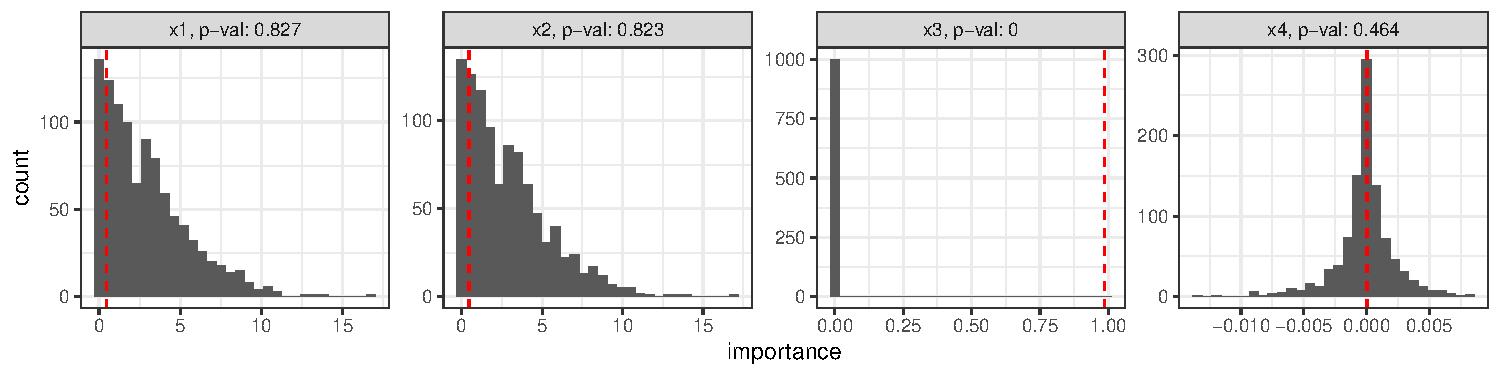
\includegraphics[width=\linewidth]{figure_man/pimp.pdf}
  %\caption{$H_0$ distribution (1000 samples) for each feature as histograms, the true PFI indicated in red. PIMP only considers $x_3$ relevant. Although PFI for $x_1$ and $x_2$ is nonzero, PIMP considers them irrelevant since they are not predictive of $y$. Even after permuting $y$, the model relies on them.}
%\end{figure}

\begin{itemize}
    \item Histograms: $H_0$ distribution of PFI scores after permuting $y$ (1000 repetitions)
    \item Red: PFI score estimated on unpermuted $y$ (under $H_1$) $\leadsto$ compare against $H_0$ distribution
    \item Results: Although PFI for $x_1$ and $x_2$ is nonzero (red), PIMP considers them not significantly relevant (p-value > 0.05) 
    %since they are not predictive of $y$
\end{itemize}
\end{frame}

\begin{frame}{Digression: Multiple testing problem \citebutton{Romano et al. (2010)}{https://doi.org/10.1057/978-1-349-95121-5_2914-1}}
\begin{itemize}[<+->]
  \item When should we reject the $H_0$-hypothesis for a feature? 
  \item The larger the number of features, the more tests need to be performed by PIMP\\
  $\leadsto$ \textbf{Multiple testing problem}: If multiplicity of tests is not taken into account, the probability that some of the true $H_0$-hypothesis is rejected (type-I error) by chance may be large
  \item Accounting for multiplicity of individual tests can be achieved by controlling an appropriate error rate, e.g., the \textbf{family-wise error rate} (FWE: probability of at least one type-I error)
  \item One classical method to control the FWE is the \textbf{Bonferroni correction} which rejects a null hypothesis if its p-value is smaller than $\alpha/m$ with $m$ as the number of performed parallel tests
  %\item We refer to other lectures or the statistics literature for more details
  \end{itemize} 

  %\footnote[frame]{\fullcite{romano2010multiple}}
  %{\tiny{Romano, J. P., Shaikh, A. M., and Wolf, M. (2010). Multiple Testing. The New Palgrave Dictionary of Economys. \url{https://home.uchicago.edu/~amshaikh/webfiles/palgrave.pdf}}\par}
\end{frame}
% \begin{frame}
%   \printbibliography
% \end{frame}

\endlecture
\end{document}
